%==============================================================================
%  Read-Only Is Not Wear-Free: The Reliability Wall of High-Bandwidth Flash
%  IEEE conference format (IEEE/ACM MICRO style, two-column IEEEtran)
%  Compile: tectonic HBF_Reliability_Paper.tex   (or pdflatex, twice)
%  References are embedded (thebibliography); no .bib file is needed.
%==============================================================================
\documentclass[conference,10pt]{IEEEtran}
\IEEEoverridecommandlockouts

\usepackage[T1]{fontenc}
\usepackage{cite}
\usepackage{amsmath,amssymb}
\usepackage{graphicx}
\usepackage{booktabs}
\usepackage{array}
\usepackage{xcolor}
\usepackage{tikz}
\usetikzlibrary{arrows.meta,positioning,calc,fit}
\usepackage{pgfplots}
\pgfplotsset{compat=1.17}
\usepackage[hidelinks]{hyperref}

% --- working notes (remove before submission) -------------------------------
% \todo{} marks a research task (a study, a model or a design to build and
% evaluate), not an editorial fix. \verify{} marks a fact to re-check.
\newcommand{\todo}[1]{\par\smallskip\noindent\fcolorbox{red}{red!4}{%
  \parbox{\dimexpr\linewidth-2\fboxsep-2\fboxrule\relax}{\footnotesize
  \textcolor{red}{\textbf{Research task.}} #1}}\par\smallskip}
\newcommand{\verify}[1]{\textcolor{orange}{[verify: #1]}}
% ----------------------------------------------------------------------------

\definecolor{cHbm}{RGB}{31,90,160}
\definecolor{cHbf}{RGB}{200,50,50}
\definecolor{cAlt}{RGB}{230,140,40}
\definecolor{cGrn}{RGB}{60,150,80}
\definecolor{cGrey}{RGB}{238,238,240}

\newcommand{\Hthree}{H\textsuperscript{3}}
\newcommand{\sys}{Steward}

\pgfplotsset{
  pp/.style={
    width=\columnwidth, height=4.4cm,
    tick label style={font=\scriptsize}, label style={font=\scriptsize},
    legend style={font=\scriptsize, draw=none, fill=none},
    grid=major, grid style={gray!25, very thin},
    every axis plot/.append style={thick, mark size=1.6pt},
  }}

\begin{document}

\title{Read-Only Is Not Wear-Free: The Reliability Wall of High-Bandwidth
Flash for LLM Inference}

\author{\IEEEauthorblockN{Garima Kalra}
\IEEEauthorblockA{\textit{Department of Computer Science and Engineering}\\
\textit{Indian Institute of Technology Guwahati}\\
k.garima@iitg.ac.in}
\and
\IEEEauthorblockN{Phrangboklang Lyngton Thangkhiew}
\IEEEauthorblockA{\textit{Department of Computer Science and Engineering}\\
\textit{Indian Institute of Technology Guwahati}}
}

\maketitle

%------------------------------------------------------------------------------
\begin{abstract}
High-Bandwidth Flash (HBF) is being proposed as the capacity tier that lets a
single GPU hold what today takes dozens: model weights and shared KV caches
that are read on every decode step but almost never written. Every published
HBF design, more than twenty in 2026 alone, rests on the same premise:
because this data is read-only, NAND's weak endurance does not matter. We
argue that the premise is wrong in exactly the regime HBF is built for. Data
that is read at a terabyte per second, next to a kilowatt GPU, for years, is
the worst case for three NAND failure mechanisms that no HBF evaluation
models together: read disturb, retention loss at high temperature, and the
error-correction and read-retry cost of keeping data correct in between. The
HBF base-die specification leaves refresh for data age and read counts to the
host, and no host-side design exists.

Using an analytical model calibrated on the \Hthree{} architecture, we show
that each static block of a ten-million-token Llama-3.1-405B deployment is
read about $5\times10^{5}$ times per day, two to six orders of magnitude
beyond published read-disturb limits over a five-year service life. Read
reclaim must rewrite the ``read-only'' tier every 11--28 minutes, which
consumes the device in 2--5 years without static wear levelling, and the
retention window itself shrinks from 24 hours to about 4 hours at a 105\,\textdegree{}C
junction. Two properties of LLM inference make this tractable: the access
schedule is known in advance, and most HBF capacity is idle, because the flash
tier is over-provisioned 17--67$\times$ for eight of nine models. We outline
\sys{}, a base-die reliability manager that exploits both, using
schedule-derived read accounting, replica rotation in spare capacity and
criticality-aware protection, and we set out the characterisation and
evaluation that would establish whether HBF can serve LLMs reliably at all.
\end{abstract}

\begin{IEEEkeywords}
high-bandwidth flash, NAND reliability, read disturb, data retention, LLM
inference, heterogeneous memory
\end{IEEEkeywords}

%==============================================================================
\section{Introduction}
%==============================================================================

Serving a large language model over a long shared context is limited by
memory capacity. At ten million tokens, the weights and pre-computed KV cache
of Llama-3.1-405B occupy 5.8\,TB, the HBM of 31 B200-class GPUs, before a single
request is admitted~\cite{ha2026h3}. High-Bandwidth Flash stacks NAND dies behind
a logic base die as HBM stacks DRAM, targeting HBM-class read bandwidth at up to
16$\times$ the capacity~\cite{sandisk2025hbf,ma2026challenges}. A base-die
specification appeared through the Open Compute Project in August
2026~\cite{ocp2026hbf}, first parts are expected in 2027~\cite{hu2026hbfsim}, and
the architecture literature has moved quickly: HBF has been chained behind HBM,
placed beside it, used to replace it, and co-designed with MoE expert streaming,
sparse attention, agentic session tiering and recommendation
serving~\cite{ha2026h3,park2026pooling,atassi2026hma,baek2026hotcold,son2026exploring,kyung2026hbfkv,peng2026grhbf,wang2026flashaccel,oliveira2026flint,kim2026dash,zhong2026hbflex,li2026hbfsucks,jonnalagadda2026splash,yin2026hbfapps,xia2026moebox}.

Nearly all of these designs share one argument. Flash is slow to write and wears
out, so it should hold data that is read-only: weights, shared prefixes,
immutable KV. \Hthree{} states that under read-only placement the weak endurance
of HBF ``is no longer a disadvantage''~\cite{ha2026h3}, and most later work
inherits the conclusion. Where papers do analyse endurance, they count
\emph{writes}, and when they disagree it is about how many writes KV caching
produces~\cite{son2026exploring,kyung2026hbfkv,baek2026hotcold,kim2026dash,wang2026flashaccel}.

\textbf{This paper argues that the read-only premise fails, and that it fails
precisely because of how HBF is meant to be used.} NAND wears through reads and
through time, not only through programs. Every read of a page slightly disturbs
the other wordlines of its block, and after enough reads the block must be
rewritten (\emph{read reclaim})~\cite{cai2015readdisturb}. Stored charge leaks,
faster at high temperature, so data must be rewritten within a retention
window~\cite{cai2017errors,luo2018heatwatch}. Between rewrites the raw bit-error
rate rises, which costs error-correction work and eventually read retries on the
critical path~\cite{cai2017errors}. These effects are mild for an SSD that
reads a block a few times an hour at 40\,\textdegree{}C. An HBF stack serving model weights
re-reads every static block on every decode step, several times per second,
sitting on an interposer next to a GPU that dissipates about a kilowatt. That is
the worst case for all three mechanisms at once.

The problem has also been assigned, by specification, to computer architects.
The OCP base-die specification leaves refresh for data age and read-disturb
counts to the host, and bounds powered-on retention at 24 hours at
85\,\textdegree{}C~\cite{ocp2026hbf,li2026hbfsucks,hu2026hbfsim}. In an SSD this work is done
by a controller with its own DRAM and firmware, hidden behind a block interface.
With HBF it must be done by the HBM base die, the GPU memory controller or the
runtime, at terabytes per second, without stalling decode. Of the proposals we
surveyed, one models read-disturb refresh for an HBF weight tier, without
temperature or error-correction cost~\cite{oliveira2026flint}; one simulator
implements retention and refresh but reports no results~\cite{hu2026hbfsim}; and
none evaluates what raw bit errors do to model accuracy, what error correction
costs at HBF bandwidth, or how any of it changes with the provisioning choices
the rest of the literature is busy making (Section~\ref{sec:gaps}).

\textbf{Problem statement.} \emph{Can a flash tier keep terabytes of read-mostly
LLM state correct, for a multi-year service life, next to a kilowatt GPU,
without giving back the capacity and bandwidth that justified it? If so, what
must the host side of the memory system do, and what does it cost?}

The answer decides whether the HBF-for-weights premise behind the whole line of
work holds. It also decides several design choices that are currently made on
other grounds: how many flash dies to provision, which cell mode to use, where
error correction lives, and whether an HBM site is worth trading for a flash
one. We make four contributions, and set out the work that remains as explicit
research tasks.

\begin{enumerate}
\item \textbf{A capacity baseline.} We extend LLMSimulator~\cite{yun2024duplex}
with a second memory tier, a batch-independent shared KV cache, context
parallelism and a block-level flash model, reproduce \Hthree{} to within 1\%, and
show that under a fixed shoreline the flash tier is over-provisioned by
17--67$\times$ for eight of nine models (Section~\ref{sec:capacity}). This
surplus becomes the key resource in the rest of the paper.
\item \textbf{The reliability wall, quantified.} We model read-disturb reclaim,
temperature-dependent retention and wear concentration for the static tier, and
show that read disturb dominates retention by 51--135$\times$, that the device
lasts 2--5 years without static wear levelling, and that the most
energy-efficient provisioning points leave no idle flash time in which to hide
reliability work (Section~\ref{sec:wall}).
\item \textbf{Two exploitable properties.} LLM inference reads its static data in
an order fixed before it runs, and most HBF capacity is unused. The first makes
per-block read and age accounting exact and free; the second can buy endurance
by replication. Replica rotation alone recovers the wear-levelled lifetime
bound without migration (Section~\ref{sec:props}).
\item \textbf{\sys{}}, a base-die reliability manager built on these properties,
and an evaluation plan covering device characterisation, thermal coupling,
accuracy under bit errors, and end-to-end serving (Sections~\ref{sec:steward}
and~\ref{sec:plan}).
\end{enumerate}

%==============================================================================
\section{Background}
%==============================================================================

\subsection{High-Bandwidth Flash}
An HBF stack places NAND core dies on a base die that holds the flash controller,
a staging buffer and the host interface. Bandwidth comes from parallelism across
many planes and dies. Published estimates for a stack range over 0.35--1.6\,TB/s
and 192\,GB--1\,TB, with array read latency between 1 and about
28\,\textmu{}s~(Table~\ref{tab:params}). The OCP specification exposes 64\,B
host reads backed by 4\,KiB NAND pages and requires writes to fill whole
pages~\cite{ocp2026hbf,li2026hbfsucks}. Most studies assume SLC cells with about
$10^{5}$ program/erase (P/E) cycles; at least one assumes TLC at roughly
$3\times10^{3}$~\cite{li2026hbfsucks}.

\subsection{NAND failure mechanisms that do not need writes}
\textit{Read disturb.} Reading a page applies a pass voltage to every other
wordline of the block, which slowly injects charge into unselected cells. Errors
accumulate with the number of reads to the block, and the standard remedy is to
reprogram the block once a read count threshold is reached, consuming a P/E
cycle~\cite{cai2015readdisturb}.

\textit{Retention.} Charge leaks from cells over time. The rate is strongly
thermally activated and is commonly modelled with an Arrhenius law; HBFSim uses
an activation energy of 1.04\,eV taken from 3D-NAND
characterisation~\cite{hu2026hbfsim,luo2018heatwatch}. Data must be rewritten
before its error rate exceeds what ECC can correct.

\textit{Error correction and read retry.} Between refreshes, the raw bit-error
rate (RBER) grows. Stronger codes and soft-decision decoding cost area, power and
latency; when a read fails to decode, the controller retries with shifted read
reference voltages, multiplying latency~\cite{cai2017errors}. At SSD bandwidths
these costs are hidden behind a block interface; at HBF bandwidths they sit on
the path of every decode step.

%==============================================================================
\section{What the Literature Assumes}
\label{sec:gaps}
%==============================================================================

We read thirty-eight papers on HBF, flash-based inference and heterogeneous LLM
memory (Section~\ref{sec:related}). Table~\ref{tab:survey} records, for the HBM+HBF
proposals, which reliability effects their evaluations model, and
Table~\ref{tab:params} the device parameters they assume.

\begin{table*}[t]
\centering
\caption{HBM+HBF proposals and the reliability effects their evaluations model.
\checkmark{} = modelled quantitatively; $\circ$ = discussed, assumed, or
implemented without results; -- = absent.}
\label{tab:survey}
\scriptsize
\setlength{\tabcolsep}{2.6pt}
\begin{tabular}{@{}l l l c c c c c c c@{}}
\toprule
\textbf{Work} & \textbf{HBF attachment} & \textbf{Static data in HBF} &
\shortstack{\textbf{Write}\\\textbf{wear}} & \shortstack{\textbf{GC /}\\\textbf{WAF}} &
\shortstack{\textbf{Wear}\\\textbf{levelling}} & \shortstack{\textbf{Read}\\\textbf{disturb}} &
\shortstack{\textbf{Retention}\\\textbf{/ temp.}} & \shortstack{\textbf{ECC /}\\\textbf{retry cost}} &
\shortstack{\textbf{Accuracy}\\\textbf{under errors}} \\
\midrule
\Hthree{}~\cite{ha2026h3} & behind HBM & weights, shared KV & $\circ$ & $\circ$ & $\circ$ & -- & -- & -- & -- \\
Pooling~\cite{park2026pooling} & behind HBM & -- (KV only) & -- & -- & $\circ$ & -- & -- & $\circ$ & -- \\
HMA~\cite{atassi2026hma} & beside HBM & experts & -- & -- & -- & -- & -- & -- & -- \\
Hot--cold~\cite{baek2026hotcold} & behind HBM & -- (idle KV) & \checkmark & $\circ$ & -- & -- & -- & -- & -- \\
Exploring~\cite{son2026exploring} & replaces HBM & weights, KV & \checkmark & -- & -- & -- & $\circ$ & -- & -- \\
KV endurance~\cite{kyung2026hbfkv} & replaces HBM & weights, KV & \checkmark & $\circ$ & $\circ$ & -- & -- & -- & -- \\
FlashAccel~\cite{wang2026flashaccel} & behind / replaces & weights, KV & \checkmark & -- & -- & -- & $\circ$ & -- & -- \\
FLINT~\cite{oliveira2026flint} & behind HBM & weights & -- & -- & -- & \checkmark & -- & -- & -- \\
DASH~\cite{kim2026dash} & direct + via HBM & weights & \checkmark & $\circ$ & -- & -- & -- & -- & -- \\
HBFlex~\cite{zhong2026hbflex} & HBF only & weights, KV & \checkmark & \checkmark & -- & -- & -- & -- & -- \\
HBF Sucks?~\cite{li2026hbfsucks} & fixed budget & weights, KV & \checkmark & $\circ$ & -- & -- & $\circ$ & -- & -- \\
HBFSim~\cite{hu2026hbfsim} & simulator & weights & -- & -- & -- & $\circ$ & $\circ$ & -- & -- \\
SPLASH~\cite{jonnalagadda2026splash} & behind HBM & evicted KV & $\circ$ & -- & -- & -- & -- & -- & -- \\
\midrule
\textbf{This work} & behind HBM & weights, shared KV & \checkmark & \checkmark & \checkmark & \checkmark\,(model) & \checkmark\,(model) & task & task \\
\bottomrule
\end{tabular}
\end{table*}

\begin{table}[t]
\centering
\caption{HBF parameters assumed in recent work.}
\label{tab:params}
\scriptsize
\setlength{\tabcolsep}{3pt}
\begin{tabular}{@{}lll@{}}
\toprule
\textbf{Parameter} & \textbf{Range} & \textbf{Examples} \\
\midrule
Read latency $t_R$ & 1--28\,\textmu{}s & 1 \cite{son2026exploring}, 3 \cite{kyung2026hbfkv}, 15 \cite{park2026pooling}, 20 \cite{ha2026h3}, 25 \cite{baek2026hotcold} \\
Program latency & 50--300\,\textmu{}s & 100 \cite{son2026exploring,kyung2026hbfkv,park2026pooling} \\
Read BW / stack & 0.35--1.6\,TB/s & 0.35 \cite{son2026exploring}, 1 \cite{ha2026h3}, 1.6 \cite{kyung2026hbfkv} \\
Capacity / stack & 192\,GB--1\,TB & 384 \cite{ha2026h3}, 512 \cite{son2026exploring}, 1024 \cite{atassi2026hma} \\
Power / stack & 30--160\,W & 30 \cite{hsu2026haven}, $<$80 \cite{son2026exploring}, 160 \cite{ha2026h3} \\
Endurance & $3.3\times10^{3}$--$10^{6}$ P/E & \cite{li2026hbfsucks}, $10^{5}$ \cite{kyung2026hbfkv}, $10^{6}$ \cite{wang2026flashaccel} \\
Read-disturb limit & $10^{3}$--$10^{6}$ reads & \cite{sun2025lincoln,oliveira2026flint} \\
Junction limit & 80--105\,\textdegree{}C & 80 \cite{li2026hbfsucks}, 105 \cite{hu2026hbfsim} \\
\bottomrule
\end{tabular}
\end{table}

The pattern is consistent. Endurance is analysed as a function of write volume,
and the disagreements between papers are about write volume: with similar KV
write rates near 1\,GB/s per GPU, one study concludes that endurance is
sufficient by assuming $10^{6}$ P/E cycles~\cite{wang2026flashaccel} and another
projects 0.645 years at $10^{5}$~\cite{kim2026dash}. Write amplification is
usually taken as 1.02, a figure that traces to a host-side SMART counter rather
than a NAND-level measurement~\cite{jeong2025hifc}. The data that the whole line
of work puts in HBF because it is \emph{safe}, weights and shared prefixes, is
the data whose reliability is not analysed. The only detailed treatment of read
disturb for LLM weights is on-device, at batch one and room temperature, where
Lincoln shows that read reclaim is affordable only with SLC, relaxed retention
and wear levelling~\cite{sun2025lincoln}. FLINT applies a similar model to an HBF
weight tier and reports a lifetime of about 29 days at $10^{5}$ P/E and 50
tokens/s, but does not model temperature, error correction or the effect of
provisioning~\cite{oliveira2026flint}.

%==============================================================================
\section{Methodology and Capacity Baseline}
\label{sec:capacity}
%==============================================================================

\subsection{Simulator}
We extend LLMSimulator~\cite{yun2024duplex}, an analytical roofline simulator
that other HBF studies also build on~\cite{son2026exploring,kyung2026hbfkv,kim2026dash}.
Each operation takes $t=\max(F/\Pi,\,t_{\mathrm{mem}})$. We split every
operation's bytes by tensor tag into $B_{\mathrm{HBM}}$ and $B_{\mathrm{HBF}}$
(weights and shared cache to flash) and compute
\begin{equation}
t_{\mathrm{mem}} =
\begin{cases}
\max\!\left(\dfrac{B_{\mathrm{HBM}}}{\beta_{\mathrm{HBM}}},\,
            \dfrac{B_{\mathrm{HBF}}}{\beta_{\mathrm{HBF}}}\right)
  & \text{partitioned,}\\[10pt]
\max\!\left(\dfrac{B_{\mathrm{HBM}}+B_{\mathrm{HBF}}}{\beta_{\mathrm{link}}},\,
            \dfrac{B_{\mathrm{HBF}}}{\beta_{\mathrm{HBF}}}\right)
  & \text{pooled.}
\end{cases}
\label{eq:tmem}
\end{equation}
We added a batch-independent shared KV tensor, a second capacity budget,
context parallelism across nodes with a corrected hierarchical all-reduce,
configurable HBM/HBF sites and dies per stack against a shoreline budget, and a
block-level flash model (4\,KiB pages, 1\,MiB blocks, DRAM write combining,
greedy collection, per-block erase counts). The changes are about 900 lines of
C++. Following \Hthree{}, we model B200 GPUs with eight 24\,GB, 1\,TB/s HBM3e cubes
and eight 384\,GB, 1\,TB/s HBF cubes, Llama-3.1-405B with FP8 weights and FP16 KV,
1K input and output tokens, and 32 GPUs across four servers at ten million
tokens. The model reproduces \Hthree{}'s batch ratio (2.71$\times$ vs.\ 2.6$\times$),
throughput (1.261$\times$ vs.\ 1.25$\times$) and throughput per watt
(0.553$\times$ vs.\ 0.548$\times$) at one million tokens, with only the batch
ratio used for calibration.

\subsection{Where the flash should go}
The capacity study determines the operating point that the reliability analysis
must work at, so we report it in some detail. With eight shoreline sites and
eight dies per stack (an HBM die holds 3\,GB, a flash die 48\,GB), the four
arrangements (Fig.~\ref{fig:arrangements}) provide the resources in
Table~\ref{tab:arrangements}.

\begin{figure*}[t]
\centering
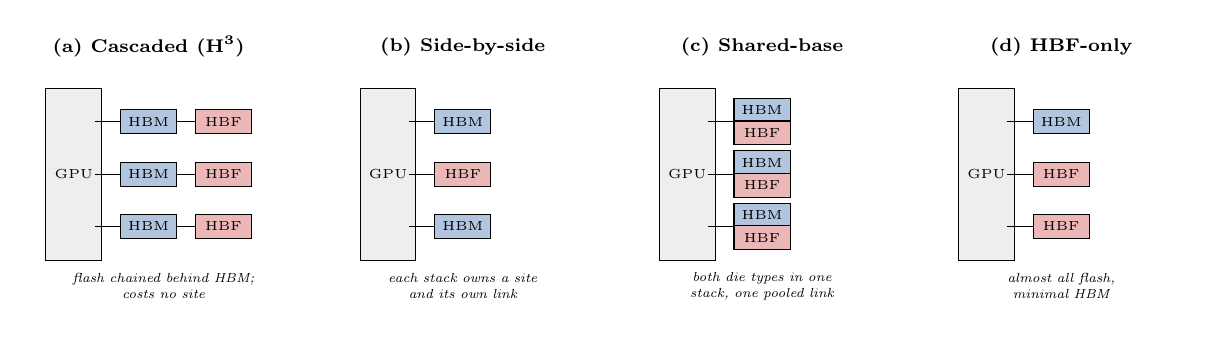
\begin{tikzpicture}[
  gpu/.style={draw, fill=cGrey, minimum width=0.55cm, minimum height=2.3cm, font=\tiny},
  hbm/.style={draw, fill=cHbm!35, minimum width=0.75cm, minimum height=0.32cm, font=\tiny, inner sep=1pt},
  hbf/.style={draw, fill=cHbf!35, minimum width=0.75cm, minimum height=0.32cm, font=\tiny, inner sep=1pt},
  hdg/.style={font=\scriptsize\bfseries},
  sub/.style={font=\tiny\itshape, text width=3.4cm, align=center},
  scale=0.95, transform shape]
\begin{scope}[xshift=0cm]
  \node[hdg] at (1.0,1.7) {(a) Cascaded (\Hthree{})};
  \node[gpu] at (0,0) {GPU};
  \foreach \y in {0.7,0,-0.7}{
    \node[hbm] at (1.0,\y) {HBM}; \node[hbf] at (2.0,\y) {HBF};
    \draw[very thin] (0.28,\y) -- (0.62,\y); \draw[very thin] (1.38,\y) -- (1.62,\y);}
  \node[sub] at (1.2,-1.5) {flash chained behind HBM;\\costs no site};
\end{scope}
\begin{scope}[xshift=4.2cm]
  \node[hdg] at (1.0,1.7) {(b) Side-by-side};
  \node[gpu] at (0,0) {GPU};
  \node[hbm] at (1.0,0.7) {HBM}; \node[hbf] at (1.0,0) {HBF}; \node[hbm] at (1.0,-0.7) {HBM};
  \foreach \y in {0.7,0,-0.7}{\draw[very thin] (0.28,\y) -- (0.62,\y);}
  \node[sub] at (1.0,-1.5) {each stack owns a site\\and its own link};
\end{scope}
\begin{scope}[xshift=8.2cm]
  \node[hdg] at (1.0,1.7) {(c) Shared-base};
  \node[gpu] at (0,0) {GPU};
  \foreach \y/\yy in {0.85/0.55, 0.15/-0.15, -0.55/-0.85}{
    \node[hbm] at (1.0,\y) {HBM}; \node[hbf] at (1.0,\yy) {HBF};
    \draw[very thin] (0.28,{(\y+\yy)/2}) -- (0.62,{(\y+\yy)/2});}
  \node[sub] at (1.0,-1.5) {both die types in one\\stack, one pooled link};
\end{scope}
\begin{scope}[xshift=12.2cm]
  \node[hdg] at (1.0,1.7) {(d) HBF-only};
  \node[gpu] at (0,0) {GPU};
  \node[hbm] at (1.0,0.7) {HBM}; \node[hbf] at (1.0,0) {HBF}; \node[hbf] at (1.0,-0.7) {HBF};
  \foreach \y in {0.7,0,-0.7}{\draw[very thin] (0.28,\y) -- (0.62,\y);}
  \node[sub] at (1.0,-1.5) {almost all flash,\\minimal HBM};
\end{scope}
\end{tikzpicture}
\caption{The four arrangements compared under an eight-site shoreline. Only the
cascaded arrangement adds flash without giving up an HBM site.}
\label{fig:arrangements}
\end{figure*}


\begin{table}[t]
\centering
\caption{Resources per GPU under an eight-site shoreline.}
\label{tab:arrangements}
\footnotesize
\setlength{\tabcolsep}{4pt}
\begin{tabular}{@{}lccccc@{}}
\toprule
\textbf{Arrangement} & \textbf{Sites} & \textbf{HBM} & \textbf{Flash} & \textbf{Link} & \textbf{TDP} \\
\midrule
Cascaded (\Hthree{}) & 8   & 192\,GB & 3072\,GB & pooled      & 2280\,W \\
Shared-base          & 8   & 96\,GB  & 1536\,GB & pooled      & 1480\,W \\
Side-by-side         & 4+4 & 96\,GB  & 1536\,GB & partitioned & 1480\,W \\
HBF-only             & 1+7 & 24\,GB  & 2688\,GB & partitioned & 1840\,W \\
\bottomrule
\end{tabular}
\end{table}

The cascade is fastest at every context length we tested, and the reason is HBM
capacity rather than flash bandwidth. At its own maximum batch it beats
shared-base by $2.45\times$; pinning both to the same request count isolates the
wiring, which contributes $1.22\times$, leaving $2.01\times$ from capacity (1457
admitted requests against 724). Re-running the cascade with half its flash still
leaves it 23\% ahead. At matched capacity, bandwidth and power, a pooled site link
beats a partitioned one by 0.7\% when flash is 70\% of capacity and by 31.7\% when
it is 99\% (Fig.~\ref{fig:pooling}), because a fixed split cannot lend bandwidth from an idle tier to a busy
one. HBF-only packages fail on concurrency, not speed: at a pinned 175 requests
they beat both shared-base and side-by-side, but 24\,GB of HBM caps them at 174
concurrent requests. Yin et al.\ reach the same qualitative ordering~\cite{yin2026hbfapps}.

\begin{figure}[t]
\centering
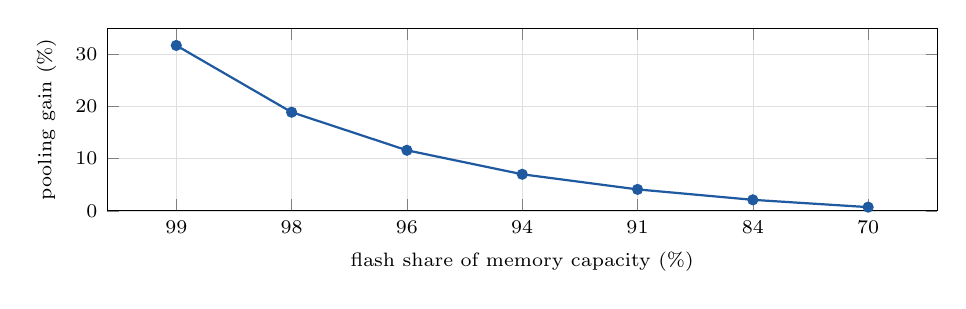
\begin{tikzpicture}
\begin{axis}[pp, height=3.9cm,
  xlabel={flash share of memory capacity (\%)}, ylabel={pooling gain (\%)},
  xtick={0,1,2,3,4,5,6},
  xticklabels={99,98,96,94,91,84,70}, ymin=0, ymax=35]
\addplot[cHbm, mark=*] coordinates {(0,31.7)(1,18.9)(2,11.6)(3,7.0)(4,4.1)(5,2.1)(6,0.7)};
\end{axis}
\end{tikzpicture}
\caption{Throughput gain of a pooled site link over a partitioned one at matched
capacity, bandwidth and power. Our pooled model charges nothing for arbitration,
so the direction of this result is built in; only its magnitude is measured.}
\label{fig:pooling}
\end{figure}

\subsection{How much flash is needed}
Flash holds only weights and the shared cache, and both follow from the model
definition (Table~\ref{tab:demand}). Eight of nine models need at most 182\,GB
per device at ten million tokens with 32-way parallelism, against 3072\,GB
provisioned: a surplus of 17--67$\times$. Only DeepSeek-V3, whose latent attention
with 128 KV heads gives a per-token footprint 7.6 times Llama's, needs more. For
five of the models flash is a prerequisite rather than an optimisation: their
shared cache alone exceeds a GPU's 192\,GB of HBM by 1.3--2.6$\times$.

\begin{table}[t]
\centering
\caption{Flash residency per device (10M tokens, 32 devices).}
\label{tab:demand}
\footnotesize
\begin{tabular}{@{}lrrr@{}}
\toprule
\textbf{Model} & \textbf{Weights} & \textbf{KV/token} & \textbf{Flash/device} \\
\midrule
Mixtral          &  93\,GB & 131\,KB &  45.9\,GB \\
Llama-4 Scout    & 216\,GB & 197\,KB &  71.2\,GB \\
Llama-4 Maverick & 801\,GB & 197\,KB &  89.5\,GB \\
Grok-1           & 633\,GB & 262\,KB & 105.7\,GB \\
OpenMoE          &  66\,GB & 393\,KB & 130.9\,GB \\
Llama-7B-MoE     &  13\,GB & 524\,KB & 172.2\,GB \\
GLaM             & 288\,GB & 524\,KB & 180.8\,GB \\
Llama-3.1-405B   & 406\,GB & 516\,KB & 181.8\,GB \\
DeepSeek-V3      & 709\,GB & 3932\,KB & 1310.7\,GB \\
\bottomrule
\end{tabular}
\end{table}

\subsection{Mixed-die stacks}
If the chained stack's capacity is unused, some of its dies can be DRAM. We keep
the front stack at eight HBM dies and write $x$H$y$F for $x$ HBM and $y$ flash
dies per site; the site link is unchanged (Table~\ref{tab:mixed}). Concurrency
rises linearly with HBM dies, because private KV is the only consumer of HBM once
static data has moved to flash, and from 8H8F to 14H2F it rises by exactly
$1.75\times$ for every model we ran. Throughput falls slowly while the pooled link
binds and quickly once the flash media binds, from 12H4F onwards, because a
constant 165.8\,GB must be read from fewer dies each step. Six of eight models
prefer 12H4F for energy efficiency; Llama-3.1-405B and DeepSeek-V3 prefer 14H2F.

\begin{table*}[t]
\centering
\caption{Mixed-die cascaded stacks, Llama-3.1-405B, 10M tokens, 32 GPUs. $T$ =
requests / tokens/s. $C/S$ = flash capacity over the 165.8\,GB static
footprint. Media util.\ = fraction of each step the flash media is busy under
Eq.~\eqref{eq:tmem}. Min.\ GPUs = smallest count whose flash holds the 5.82\,TB
static footprint.}
\label{tab:mixed}
\footnotesize
\begin{tabular}{@{}lrrrrrrrrrr@{}}
\toprule
\textbf{Design} & \textbf{HBM} & \textbf{Flash} & \textbf{Requests} & \textbf{Tok/s} &
\textbf{Tok/s/W} & \textbf{TDP} & \textbf{$T$ (ms)} & \textbf{$C/S$} &
\textbf{Media util.} & \textbf{Min.\ GPUs} \\
\midrule
8H8F  & 192\,GB & 3072\,GB & 1457 & 8881 & 0.1218 & 2280\,W & 164 & 18.5 & 64\%  & 2 \\
10H6F & 240\,GB & 2304\,GB & 1824 & 8839 & 0.1354 & 2040\,W & 206 & 13.9 & 78\%  & 3 \\
12H4F & 288\,GB & 1536\,GB & 2191 & 8579 & 0.1489 & 1800\,W & 255 &  9.3 & 100\% & 4 \\
14H2F & 336\,GB &  768\,GB & 2557 & 7721 & 0.1547 & 1560\,W & 331 &  4.6 & 100\% & 8 \\
15H1F & 360\,GB &  384\,GB & 2741 & 6380 & 0.1384 & 1440\,W & 430 &  2.3 & 100\% & 16 \\
\bottomrule
\end{tabular}
\end{table*}

\subsection{The efficiency and GPU-count consequences are conditional}
The TDP column uses \Hthree{}'s assumption of 160\,W per HBF cube. Other work
assumes less than 80\,W~\cite{son2026exploring,peng2026grhbf} or budgets 30\,W per
stack~\cite{hsu2026haven}. Because throughput in our model does not depend on
power, the same throughputs can be re-divided by the TDP each assumption implies
(Fig.~\ref{fig:power}). 12H4F beats 8H8F on tokens per joule only if an HBF cube
draws more than about 52\,W; the thresholds for 10H6F and 14H2F are 43\,W and
75\,W. Removing flash dies also raises the minimum GPU count: 8H8F holds the
static data on two GPUs, as \Hthree{} claims, but 12H4F needs four and 14H2F eight.
The concurrency gain holds regardless of power.

\begin{figure}[t]
\centering
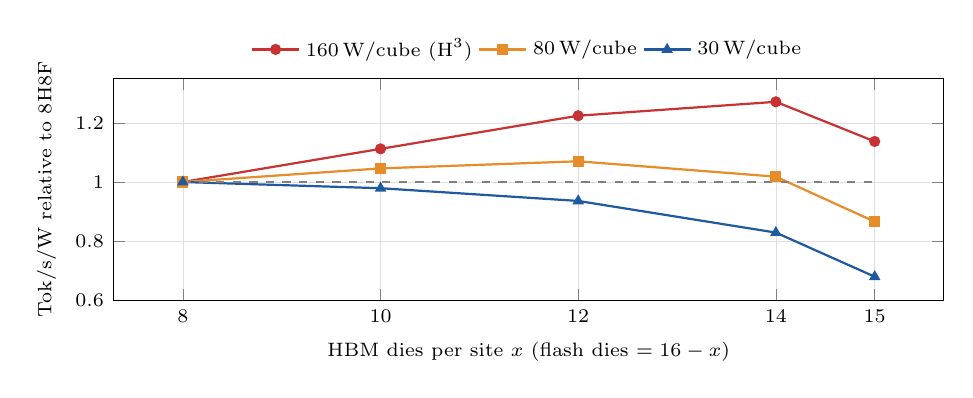
\begin{tikzpicture}
\begin{axis}[pp,
  xlabel={HBM dies per site $x$ (flash dies $=16-x$)},
  ylabel={Tok/s/W relative to 8H8F},
  xtick={8,10,12,14,15}, ymin=0.6, ymax=1.35,
  legend style={at={(0.5,1.03)}, anchor=south, legend columns=3}]
\addplot[cHbf, mark=*] coordinates {(8,1.000)(10,1.112)(12,1.224)(14,1.271)(15,1.137)};
\addlegendentry{160\,W/cube (\Hthree{})}
\addplot[cAlt, mark=square*] coordinates {(8,1.000)(10,1.046)(12,1.070)(14,1.018)(15,0.866)};
\addlegendentry{80\,W/cube}
\addplot[cHbm, mark=triangle*] coordinates {(8,1.000)(10,0.979)(12,0.936)(14,0.829)(15,0.680)};
\addlegendentry{30\,W/cube}
\addplot[gray, dashed, thin, mark=none] coordinates {(8,1)(15,1)};
\end{axis}
\end{tikzpicture}
\caption{Energy efficiency of mixed-die stacks under three HBF power
assumptions. Throughput is unchanged; only the TDP differs.}
\label{fig:power}
\end{figure}

\subsection{What this means for reliability}
Two columns of Table~\ref{tab:mixed} matter for the rest of the paper. $C/S$ is the
idle \emph{capacity} available for reliability, and media utilisation the idle
flash \emph{time}. The designs that are most attractive for concurrency and energy
have neither. This is the tension the rest of the paper examines.

%==============================================================================
\section{The Reliability Wall}
\label{sec:wall}
%==============================================================================

\subsection{Read pressure on static data}
A decode step streams the whole static footprint once. At the step times of
Table~\ref{tab:mixed}, each static block is read in $2.0$--$5.3\times10^{5}$
steps per day, and $3.7$--$9.6\times10^{8}$ steps over five years. Published
read-disturb limits range from $10^{3}$ to $10^{6}$ reads per
block~\cite{sun2025lincoln,oliveira2026flint}. Every static block therefore
crosses its read-disturb limit hundreds to about a million times in its service
life, and must be rewritten each time. Batching does not help: weights are read
once per step regardless of how many requests share the step.

\subsection{A reclaim model}
Let $T$ be the step time, $k$ the page reads a block receives per step, $R$ the
read-disturb threshold, $\tau_{\mathrm{ret}}$ the retention window, $S$ the
static footprint and $C$ the flash capacity. A block must be reclaimed every
\begin{equation}
\tau = \min\!\left(\frac{R\,T}{k},\; \tau_{\mathrm{ret}}(\Theta)\right),
\label{eq:tau}
\end{equation}
where $\Theta$ is the die temperature. If reclaim writes land in the static
region, lifetime is $L_{0}=N_{\mathrm{PE}}\,\tau$; if a static wear leveller
spreads them over the device, $L_{\mathrm{WL}}=N_{\mathrm{PE}}\,\tau\,C/S$.

With FLINT-like parameters ($R=10^{6}$ page reads per block, $k=256$ pages per
1\,MiB block, $10^{5}$ P/E), $\tau$ is 11--28 minutes across the designs of
Table~\ref{tab:mixed}. The refresh write traffic is small, 99--259\,MB/s per
device, so this is not a bandwidth problem. It is an endurance problem:
$L_{0}$ is 2.0--5.3 years, and only the slowest design reaches a five-year
service target (Fig.~\ref{fig:life}). With ideal static wear levelling,
$L_{\mathrm{WL}}$ is 12--38 years. The ordering of designs reverses between the
two: without levelling, $L_{0}\propto T$ and removing flash dies helps because
each step is slower; with levelling, $L_{\mathrm{WL}}\propto T\,C$ and removing
flash dies hurts.

\subsection{Temperature}
The OCP retention bound of 24 hours applies at 85\,\textdegree{}C. With the 1.04\,eV
activation energy used by HBFSim~\cite{hu2026hbfsim,luo2018heatwatch}, the same
data retains for about 9.6 hours at 95\,\textdegree{}C and 4.0 hours at 105\,\textdegree{}C, the
junction limit HBFSim assumes; at 55\,\textdegree{}C it would retain for three weeks
(Fig.~\ref{fig:temp}). Under the FLINT-like parameters read disturb still sets
$\tau$ at every temperature in this range, by a factor of 9--22 at 105\,\textdegree{}C and
51--135 at 85\,\textdegree{}C across the designs. Two things change the picture, and neither has been
studied. First, read disturb itself is temperature dependent, so $R$ is a
function of $\Theta$. Second, an HBF stack is not isothermal: dies closer to the
base die and to the GPU run hotter, so different dies of one stack age at
different rates and a single refresh policy is wrong for most of them.

\begin{figure}[t]
\centering
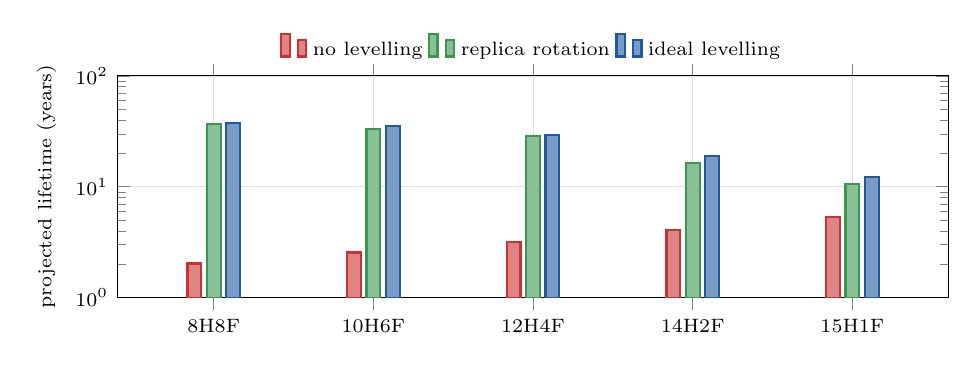
\begin{tikzpicture}
\begin{axis}[pp, ybar, bar width=5pt, ymode=log, log origin=infty,
  ylabel={projected lifetime (years)},
  symbolic x coords={8H8F,10H6F,12H4F,14H2F,15H1F}, xtick=data,
  ymin=1, ymax=100,
  legend style={at={(0.5,1.02)}, anchor=south, legend columns=3},
  enlarge x limits=0.15]
\addplot[fill=cHbf!60, draw=cHbf] coordinates
  {(8H8F,2.03)(10H6F,2.56)(12H4F,3.16)(14H2F,4.10)(15H1F,5.32)};
\addlegendentry{no levelling}
\addplot[fill=cGrn!60, draw=cGrn] coordinates
  {(8H8F,36.6)(10H6F,33.2)(12H4F,28.5)(14H2F,16.4)(15H1F,10.6)};
\addlegendentry{replica rotation}
\addplot[fill=cHbm!60, draw=cHbm] coordinates
  {(8H8F,37.7)(10H6F,35.5)(12H4F,29.3)(14H2F,19.0)(15H1F,12.3)};
\addlegendentry{ideal levelling}
\end{axis}
\end{tikzpicture}
\caption{Lifetime of the static tier under read-disturb reclaim alone
($R=10^{6}$, $k=256$, $10^{5}$ P/E). Replica rotation
(Section~\ref{sec:props}) reaches the ideal levelling bound without
migrating data.}
\label{fig:life}
\end{figure}

\begin{figure}[t]
\centering
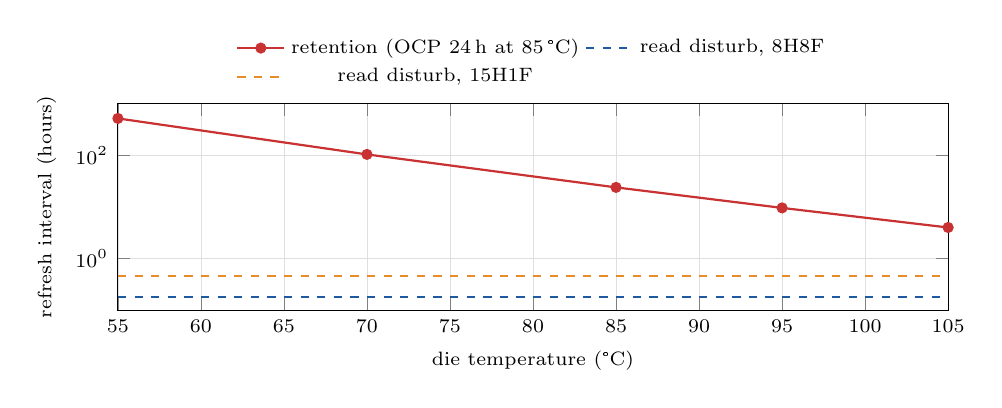
\begin{tikzpicture}
\begin{axis}[pp, ymode=log, height=4.2cm,
  xlabel={die temperature (\textdegree{}C)}, ylabel={refresh interval (hours)},
  xmin=55, xmax=105, ymin=0.1, ymax=1000,
  legend style={at={(0.5,1.03)}, anchor=south, legend columns=2}]
\addplot[cHbf, mark=*] coordinates {(55,522.6)(70,104.7)(85,24.0)(95,9.6)(105,4.0)};
\addlegendentry{retention (OCP 24\,h at 85\,\textdegree{}C)}
\addplot[cHbm, dashed, mark=none] coordinates {(55,0.178)(105,0.178)};
\addlegendentry{read disturb, 8H8F}
\addplot[cAlt, dashed, mark=none] coordinates {(55,0.466)(105,0.466)};
\addlegendentry{read disturb, 15H1F}
\end{axis}
\end{tikzpicture}
\caption{Refresh interval set by retention (Arrhenius, $E_a=1.04$\,eV) and by
read disturb ($R=10^{6}$, $k=256$, taken as temperature-independent here). The
temperature dependence of read disturb is one of the open questions.}
\label{fig:temp}
\end{figure}

\subsection{Wear concentration}
The static region is not the only one that wears. When HBM is over-subscribed
and private KV spills to flash, the spill region cycles continuously while the
static region, absent reclaim, never does. In our block-level model, the spill
region of 8H8F lasts 0.5 years without static wear levelling and 5.7 years with
it, a factor of 10.7; the factor is 5.0 for 12H4F and 2.2 for 14H2F, because
less spare capacity is available to spread the wear. KV garbage collection
itself is nearly free under per-request allocation (victim blocks are fully
invalid, WAF 1.33 from buffer flushes alone), because a request's KV dies all
at once. Read reclaim and spill wear draw on the same P/E budget, and no study
has combined them.

\subsection{No idle time}
In an SSD, refresh and retries hide in idle time. Under Eq.~\eqref{eq:tmem},
the flash media of 8H8F is busy 64\% of each decode step, which leaves room for
reclaim programs and re-reads. From 12H4F onwards the media is the bottleneck
and is busy for the entire step (Table~\ref{tab:mixed}). Any reliability work
then comes directly out of decode throughput, and every read retry extends the
step. The provisioning choices that the capacity study favours are exactly the
ones that remove the slack reliability management needs.

\subsection{What is not yet known}
The model above bounds only the refresh-driven wear. Three larger unknowns
remain, and each could move the conclusion in either direction.

\todo{\textbf{Error-rate model for HBF under LLM access patterns.} Build an RBER
model as a joint function of P/E count, reads since last program, time since
program and temperature, calibrated against published 3D-NAND characterisation
for SLC and pSLC-mode TLC~\cite{cai2015readdisturb,cai2017errors,luo2018heatwatch}.
Replace the fixed threshold $R$ with the read count at which RBER crosses the
correction limit of a chosen code, and report $\tau$, lifetime and refresh
traffic as distributions rather than points. Establish whether the $10^{3}$ and
$10^{6}$ thresholds used in the literature are for comparable cells, page sizes
and temperatures, and which applies to HBF's shrunk, many-plane arrays.}

\todo{\textbf{Thermal coupling of an HBF stack to the GPU.} Derive a per-die
temperature map of a flash stack chained behind HBM next to a B200-class GPU
under decode power, using a compact thermal model (e.g., the 3D-ICE based models
of~\cite{li2026hbfsucks,hu2026hbfsim}) and the power cases of
Table~\ref{tab:params}. Feed per-die temperatures into the error model to obtain
per-die refresh deadlines, and quantify how much of the stack ages faster than
the average. Determine whether cascaded, side-by-side and shared-base placement
differ materially in flash temperature, which would add a reliability term to
the topology comparison.}

\todo{\textbf{Error-correction and read-retry cost at HBF bandwidth.} Size BCH and
LDPC decoders for 1--1.6\,TB/s per stack on the base die (area, power, latency)
across the RBER range the error model predicts, including parity overhead on the
link. Model read-retry probability as RBER grows between refreshes, its effect
on the latency-hiding buffer of \Hthree{}, and the resulting tail of decode step
time and TPOT. Identify the refresh interval that minimises total cost: wear
from refreshing early against decode power and latency from correcting late.}

%==============================================================================
\section{Two Properties Worth Exploiting}
\label{sec:props}
%==============================================================================

\subsection{The access schedule is known in advance}
An SSD controller must count reads per block because its workload is
unpredictable. LLM decode is not. The static region is streamed in the same
layer order every step, each block receives the same $k$ page reads per step,
and the step count is known to the runtime. Per-block read counts and ages are
therefore a function of a single counter and a static layout table. This removes
per-block read counters, makes every refresh deadline exact rather than
conservative, and tells the controller when each block will next be read, so a
reclaim can be scheduled immediately after the last read before its deadline and
the fresh copy used from the next step on. The same knowledge predicts the
threshold-voltage drift of each block, which allows read reference voltages to be
preset from age and read count instead of discovered through
retries~\cite{cai2017errors}.

\subsection{Most of the capacity is idle}
Section~\ref{sec:capacity} showed that $C/S$ ranges from 2.3 to 18.5. Storing
$r\le\lfloor C/S\rfloor$ copies of the static data and rotating which copy each
step reads divides the read rate per physical block by $r$, so $\tau$ and $L_{0}$
grow by $r$. Replica rotation moves no data after the initial write, yet reaches
97\% of the ideal wear-levelled lifetime for 8H8F and 12H4F and 86\% for 14H2F
(Fig.~\ref{fig:life}). The same replicas spread read load across plane groups,
which HBFlex already does for hot prefixes to balance
bandwidth~\cite{zhong2026hbflex}, and give a second copy to fall back on when a
read fails to decode, turning a read retry into a read from another replica.
This reframes the over-provisioning result: capacity that is waste for
performance is a reliability budget. It also changes the die-split question,
because every flash die removed to gain concurrency removes replicas.

\todo{\textbf{Capacity-for-reliability trade space.} Formulate the allocation of
spare HBF capacity among replicas, pSLC-mode conversion of TLC dies (lower
density, several times the endurance and lower read latency), spill space for
over-subscribed KV and stronger ECC parity, as an optimisation with lifetime,
throughput and GPU count as objectives. Solve it per model and context length,
and determine whether the answer changes the recommended die split of
Section~\ref{sec:capacity}. Include the DeepSeek-V3 case, where the flash tier is
not over-provisioned and the budget is near zero.}

%==============================================================================
\section{\sys{}: A Base-Die Reliability Manager}
\label{sec:steward}
%==============================================================================

\sys{} is the host-side counterpart that the OCP specification assumes but does
not define. It sits on the HBM base die of a cascaded stack, between the GPU
link and the downstream HBF link, next to the address router and
latency-hiding buffer that \Hthree{} already places there (Fig.~\ref{fig:steward}).

\begin{figure}[t]
\centering
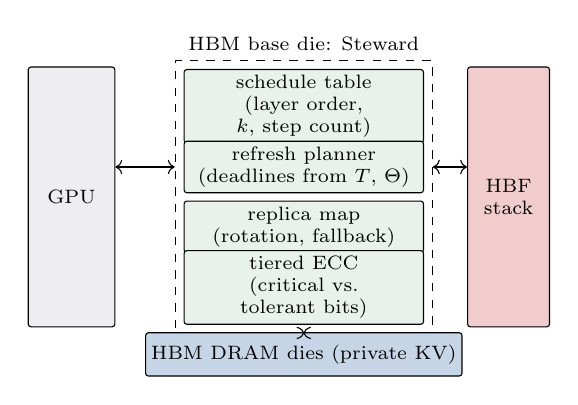
\begin{tikzpicture}[
  box/.style={draw, rounded corners=1pt, font=\scriptsize, align=center,
              minimum height=0.55cm, inner sep=2pt},
  unit/.style={box, fill=cGrn!12, text width=2.9cm},
  arr/.style={-{Latex[length=1.6mm]}, thin}]
\node[box, fill=cGrey, minimum width=1.1cm, minimum height=3.3cm] (gpu) at (0,0) {GPU};
\node[unit] (s1) at (2.95,1.15) {schedule table\\(layer order, $k$, step count)};
\node[unit] (s2) at (2.95,0.38) {refresh planner\\(deadlines from $T$, $\Theta$)};
\node[unit] (s3) at (2.95,-0.38) {replica map\\(rotation, fallback)};
\node[unit] (s4) at (2.95,-1.15) {tiered ECC\\(critical vs.\ tolerant bits)};
\node[draw, dashed, fit=(s1)(s4), inner sep=3pt, label={[font=\scriptsize]above:HBM base die: \sys{}}] (bd) {};
\node[box, fill=cHbf!25, minimum width=1.0cm, minimum height=3.3cm, text width=0.9cm] (hbf) at (5.55,0) {HBF\\stack};
\node[box, fill=cHbm!25, minimum width=2.9cm, font=\scriptsize] (dram) at (2.95,-2.0) {HBM DRAM dies (private KV)};
\draw[arr, <->] (gpu.east |- s2) -- (bd.west |- s2);
\draw[arr, <->] (bd.east |- s2) -- (hbf.west |- s2);
\draw[arr, <->] (dram.north) -- (bd.south);
\end{tikzpicture}
\caption{\sys{} on the base die of a cascaded HBM stack.}
\label{fig:steward}
\end{figure}

\textit{Schedule table and refresh planner.} The runtime registers the static
layout (which blocks each layer reads, in which order) and signals step
boundaries. The planner derives each block's read count and age, combines them
with the per-die temperature, and issues reclaims just after a block's last read
before its deadline, preferring steps in which the flash media has slack.
Where the media has no slack (12H4F and below), it places reclaims where they
delay the fewest subsequent reads.

\textit{Replica map.} Static data is written $r$ times at load. The map rotates
the replica each step reads, retires replicas as they approach their deadline
and redirects reads to a sibling when decoding fails.

\textit{Tiered protection.} Not every bit of a weight matters equally: sign and
exponent bits of FP8 and BF16 values, and the outlier channels that quantisation
work treats specially, are far more sensitive than low mantissa bits. \sys{}
applies a strong code to the sensitive portion and a light code to the rest,
reducing decoder power at terabytes per second, and allows tolerant data to run
closer to its correction limit before refresh.

\todo{\textbf{Design and evaluate \sys{} end to end.} Specify the schedule table,
planner, replica map and tiered codes in enough detail to estimate base-die area
and power against the budget left after the \Hthree{} latency-hiding buffer (about
6.7\% of a 121\,mm$^2$ die). Implement them in the simulator with the error and
thermal models of Section~\ref{sec:wall}, and compare lifetime, throughput,
TPOT tail and energy against (a) no management, (b) conventional SSD-style
per-block counters with threshold reclaim, and (c) FLINT's refresh
scheme~\cite{oliveira2026flint}. Quantify how much each mechanism contributes.}

\todo{\textbf{Accuracy under raw bit errors.} Inject bit errors into weights and
shared KV of representative models (dense, MoE and latent attention; FP8 and
BF16) at the RBERs the error model predicts between refreshes, and measure
accuracy on long-context and reasoning benchmarks. Determine which bits, tensors
and layers are critical, whether errors in the shared KV cache behave differently
from errors in weights, and what residual error rate is acceptable after tiered
correction. This defines how much protection and how much refresh \sys{} can
safely remove.}

%==============================================================================
\section{Evaluation Plan}
\label{sec:plan}
%==============================================================================

The research tasks above produce models; this section states how they will be
combined into an answer to the problem statement.

\todo{\textbf{Reliability-aware provisioning study.} Repeat the capacity study of
Section~\ref{sec:capacity} with lifetime as a constraint: for each model, context
length and service target (3 and 5 years), find the die split, cell mode, replica
count and GPU count that maximise throughput per dollar. Report where the
reliability constraint changes the answer relative to a performance-only study,
including whether side-by-side or HBF-only packages become preferable once
temperature and slack are counted.}

\todo{\textbf{Workload realism.} Replace the single input/output length with
real traces (conversational, long-document and agentic sessions) and heavy-tailed
request lengths; include prefill, corpus updates to the shared cache (which
create genuine overwrite traffic), model swaps and multi-tenant serving, all of
which change the read and write pressure on the static tier.}

\todo{\textbf{Validation beyond the analytical model.} Check the timing
consequences of refresh and retries against a cycle-level HBF model
(HBF-Sim~\cite{li2026hbfsim}) and the refresh and thermal behaviour against
HBFSim~\cite{hu2026hbfsim}; compare with DASH~\cite{kim2026dash}, which extends
the same base simulator. Where possible, measure read-disturb and retention
behaviour on commercial SLC or low-latency NAND at elevated temperature to
calibrate the error model.}

\todo{\textbf{Adversarial read pressure.} In multi-tenant deployments one tenant
controls part of the access stream. Analyse whether concentrated reads can raise
the error rate of another tenant's weights faster than the refresh plan assumes,
in the spirit of disturbance studies on DRAM and 3D NAND, and whether the
schedule-based planner can detect and bound it.}

%==============================================================================
\section{Discussion}
%==============================================================================

\textit{Why this matters beyond HBF.} The read-only premise is attractive because
it seems to remove the hard part of flash. If it does not hold at HBF's
operating point, the consequences reach every proposal that puts weights or
prefixes in flash, and the choice of what to store in HBF becomes a reliability
decision as much as a performance one. If \sys{}-style management makes it hold
cheaply, it gives the specification's host-managed refresh contract a concrete
implementation.

\textit{Limitations of the current analysis.} Our lifetimes use a fixed read
threshold and an Arrhenius retention model with one activation energy; they
bound the problem rather than predict it. The capacity study is analytical and
ignores latency, which matters once retries appear. The specification details we
rely on are taken from their descriptions in other papers and must be confirmed
against the document itself~\cite{ocp2026hbf}.

%==============================================================================
\section{Related Work}
\label{sec:related}
%==============================================================================

\textit{HBM with HBF.} \Hthree{} introduced read-only placement behind
HBM~\cite{ha2026h3}. Later designs add custom base dies for KV
staging~\cite{park2026pooling}, hardware expert migration~\cite{atassi2026hma},
hot--cold session tiering~\cite{baek2026hotcold}, burst-coalescing and refresh
hiding for weights~\cite{oliveira2026flint}, direct and relayed
paths~\cite{kim2026dash}, HBF-only packages with lifetime-aware
reclamation~\cite{zhong2026hbflex}, sparse attention over HBF-resident
KV~\cite{jonnalagadda2026splash}, expert replication and multi-model
residency~\cite{yin2026hbfapps}, and appliance-level provisioning of DRAM and
host bandwidth~\cite{xia2026moebox}. Characterisation studies examine HBF as main
memory~\cite{son2026exploring}, KV endurance through read-to-write
ratios~\cite{kyung2026hbfkv}, write-aware admission for
recommendation~\cite{peng2026grhbf} and full-stack costs~\cite{li2026hbfsucks}.
Simulators~\cite{hu2026hbfsim,li2026hbfsim}, layout~\cite{ju2026tilelens} and
other applications~\cite{hsu2026haven} complete the picture. Ma and Patterson list
HBF among four directions for inference hardware~\cite{ma2026challenges}.

\textit{Flash for LLMs.} LLM in a Flash, AiF, Lincoln and Cambricon-LLM run
single-batch inference from on-device
flash~\cite{alizadeh2024llmflash,lee2025aif,sun2025lincoln,yu2024cambriconllm};
Lincoln's read-reclaim analysis is the closest precedent for ours. ZnG placed
Z-NAND next to GPU cores~\cite{zhang2020zng}. Storage-side systems offload KV or
computation to SSDs~\cite{jeong2025hifc,pan2025instattention,jang2026hilos,jang2024smartinfinity}.

\textit{NAND reliability.} Read disturb, retention and their mitigation are well
characterised for SSDs~\cite{cai2015readdisturb,cai2017errors,luo2018heatwatch,liu2012retention}.
What is new here is the operating point, a static region read several times per
second at GPU temperatures, and a host that knows its access schedule exactly.

\textit{Other heterogeneous memory.} H2M2, LIA, CENT and Stratum tier LLM data
across byte-addressable, write-tolerant
memories~\cite{hwang2025h2m2,kim2025lia,gu2025cent,pan2025stratum}; RoMe and
InfiniGen address access granularity and KV
prefetch~\cite{nam2026rome,lee2024infinigen}.

%==============================================================================
\section{Conclusion}
%==============================================================================

HBF promises to replace dozens of GPUs bought for capacity with a flash tier that
holds read-only data. Our analysis indicates that ``read-only'' is not a
reliability property at HBF's operating point: every static block is read two to
six orders of magnitude more often than its read-disturb limit over a service
life, the retention window shrinks to hours at GPU temperatures, and the
provisioning points that look best for performance leave no time or capacity to
manage either. The same workload that creates the problem also offers a way out,
because its access schedule is known and most of its flash capacity is idle. The
work set out here, an error model, thermal coupling, correction cost, accuracy
under errors and the \sys{} manager built on them, is what it would take to know
whether HBF can hold LLM state reliably, and at what price.

%==============================================================================
\section*{Acknowledgment}
%==============================================================================
We thank the SNU SCALE lab for releasing LLMSimulator. Generative AI tools were
used to help organise the literature survey and to edit the language of this
manuscript. The simulator extensions, experiments, analysis and conclusions are
the authors' own, and the authors take full responsibility for the content.

%==============================================================================
\begin{thebibliography}{99}
%==============================================================================

\bibitem{ha2026h3}
M.~Ha, E.~Kim, and H.~Kim, ``{H$^3$}: Hybrid architecture using high bandwidth
memory and high bandwidth flash for cost-efficient {LLM} inference,''
\emph{IEEE Comput. Archit. Lett.}, vol.~25, no.~1, pp.~49--52, 2026,
doi: 10.1109/LCA.2026.3660969.

\bibitem{park2026pooling}
J.~Park, H.~An, H.~Suh, Y.~Yoon, H.~Lee, and J.~Kim, ``{HBM-HBF}-centric memory
pooling architecture with custom base die for terabyte-scale {LLM} inference,''
\emph{IEEE Comput. Archit. Lett.}, vol.~25, no.~2, pp.~259--262, 2026,
doi: 10.1109/LCA.2026.3703982.

\bibitem{atassi2026hma}
H.~Atassi, N.~Zilberman, and A.~Awad, ``Hardware-managed heterogeneous
high-bandwidth memory and flash in {LLM} inference systems,'' Univ. of Oxford
Research Archive, 2026. [Online]. Available:
\url{https://ora.ox.ac.uk/objects/uuid:a9f80041-ff2e-4714-9bc4-51c513604d36}
\verify{venue}

\bibitem{baek2026hotcold}
J.~Baek, W.~Ji, S.~Yoo, and J.-Y.~Kim, ``Hot--cold tiering of {HBM} and high
bandwidth flash for agentic {LLM} serving,'' arXiv:2609.25782, 2026.

\bibitem{son2026exploring}
D.~Son, Y.~Park, H.~Cho, H.~Ham, O.~Mutlu, S.~Lee, G.~Kim, and J.~Park,
``Exploring high-bandwidth flash for modern {LLM} inference: Opportunities and
challenges,'' \emph{IEEE Comput. Archit. Lett.}, vol.~25, no.~2, pp.~251--254,
2026, doi: 10.1109/LCA.2026.3705817.

\bibitem{kyung2026hbfkv}
K.~Kyung, Y.~J.~Moon, J.~Cho, and J.~H.~Ahn, ``High-bandwidth flash for {KV}
caches: Endurance and performance implications,'' \emph{IEEE Comput. Archit.
Lett.}, vol.~25, no.~1, pp.~210--213, 2026, doi: 10.1109/LCA.2026.3695938.

\bibitem{peng2026grhbf}
D.~Peng, K.~Wu, T.~Zuo, P.~Xia, and H.~Zang, ``Enabling high-bandwidth flash
for generative recommendation serving with write-aware {KV} cache policy,''
arXiv:2609.07175, 2026.

\bibitem{wang2026flashaccel}
X.~Wang, Y.~Xue, X.~Sun, X.~Zhang, C.~Dou, X.~Li, and X.~Chen, ``{FlashAccel}:
Leveraging high-bandwidth flash for high-throughput {LLM} inference,''
arXiv:2607.10186, 2026.

\bibitem{oliveira2026flint}
G.~F.~Oliveira, A.~Tavakkol, X.~Zhu, A.~C.~Y{\"u}z{\"u}g{\"u}ler,
V.~Arulchelvan, L.~Cavigelli, R.~Andri, M.~Sadrosadati, X.~Jia, O.~Mutlu,
K.~Zhou, S.~Bergman, and J.~Zhang, ``{FLINT}: Efficiently leveraging high
bandwidth flash for capacity-scalable {LLM} inference acceleration,''
arXiv:2608.25062, 2026.

\bibitem{kim2026dash}
S.~Kim, J.~Jin, and J.-Y.~Kim, ``Beyond capacity: Scalable {MoE} {LLM}
inference via high-bandwidth flash with direct {GPU} and {HBM} paths,''
arXiv:2608.14333, 2026.

\bibitem{zhong2026hbflex}
S.~Zhong, W.~Xu, Y.~Zhou, T.~Zhao, T.~Zhao, Y.~Kang, C.~Chang, S.~Li, G.~Sun,
and M.~Li, ``{HBFlex}: A flexible memory system for bridging fine-grained {LLM}
states and coarse-grained {HBF} parallel execution,'' arXiv:2609.18675, 2026.

\bibitem{li2026hbfsucks}
Z.~Li, Z.~Bian, X.~Huang, Y.~Zhao, G.~Sun, and Y.~Zhuo, ``{HBF} sucks? {A}
full-stack characterization of high-bandwidth flash for {KV}-centric {LLM}
serving,'' arXiv:2608.11668, 2026.

\bibitem{hu2026hbfsim}
Y.~Hu, Y.~Yang, Y.~Zhu, K.~Chu, Y.~Zheng, A.~Quinn, and W.~Zhang, ``{HBFSim}:
Fast and faithful simulation of high-bandwidth flash under real {GPU}
execution,'' arXiv:2609.09800, 2026.

\bibitem{li2026hbfsim}
Y.~Li, J.~Wang, J.~Wang, L.~Yang, H.~Yan, X.~Chai, and L.~Shi, ``{HBF-Sim}: An
extensible {HBF} simulator for large-scale {GPU} memory systems,''
arXiv:2609.29246, 2026.

\bibitem{ju2026tilelens}
J.~H.~Ju, E.~Chung, H.~Taneja, A.~Saxena, S.~Jeong, H.~Kim, and M.~K.~Qureshi,
``{TileLens}: Efficiently using large-granularity memory systems with
transparent two-dimensional memory layout,'' arXiv:2607.04031, 2026.

\bibitem{hsu2026haven}
P.-K.~Hsu, W.~Xu, Q.~Liu, T.~Rosing, and S.~Yu, ``{HAVEN}: High-bandwidth flash
augmented vector engine for large-scale approximate nearest-neighbor search
acceleration,'' arXiv:2603.01175, 2026.

\bibitem{jonnalagadda2026splash}
A.~A.~Jonnalagadda, A.~Haputhanthri, P.~Dangi, R.~Juneja, W.~Yue, A.~Bagchi,
B.~Gao, T.~Mitra \emph{et al.}, ``{SPLASH}: Co-designing sparse attention with
high-bandwidth flash for efficient long-context inference,''
arXiv:2609.23816, 2026. \verify{complete author list}

\bibitem{yin2026hbfapps}
Y.~Yin, Y.~Zhao, Z.~Yun, G.~Wu, F.~Zhu, K.~Tao, S.~Li, F.~Huang, Z.~Zhang,
S.~Li, and H.~Zheng, ``Potential applications of {HBF} in {LLM} serving
systems,'' arXiv:2608.13127, 2026.

\bibitem{xia2026moebox}
P.~Xia, T.~Hao, S.~Li, J.~Chen, S.~Wei, W.~Zou, R.~Zhang, and H.~Zang,
``Trillion-parameter {MoE} in a box: Decoupling memory provisioning with
high-bandwidth flash,'' arXiv:2609.15636, 2026.

\bibitem{ma2026challenges}
X.~Ma and D.~Patterson, ``Challenges and research directions for large
language model inference hardware,'' arXiv:2601.05047, 2026.

\bibitem{ocp2026hbf}
Open Compute Project, ``High bandwidth flash high-level base die
specification,'' Tech. Rep., version 0.7.0, Aug. 2026. \verify{full URL; confirm
the refresh and retention clauses in the document itself}

\bibitem{sandisk2025hbf}
Sandisk, ``Sandisk {HBF} fact sheet,'' 2025. [Online]. Available:
\url{https://documents.sandisk.com/content/dam/asset-library/en_us/assets/public/sandisk/collateral/company/Sandisk-HBF-Fact-Sheet.pdf}

\bibitem{yun2024duplex}
S.~Yun \emph{et al.}, ``Duplex: A device for large language models with mixture
of experts, grouped query attention, and continuous batching,'' in \emph{Proc.
57th IEEE/ACM Int. Symp. Microarchitecture (MICRO)}, 2024.
\verify{author list and pages}

\bibitem{alizadeh2024llmflash}
K.~Alizadeh, S.~I.~Mirzadeh, D.~Belenko, S.~K.~Khatamifard, M.~Cho,
C.~C.~Del~Mundo, M.~Rastegari, and M.~Farajtabar, ``{LLM} in a flash: Efficient
large language model inference with limited memory,'' in \emph{Proc. 62nd
Annu. Meeting Assoc. Comput. Linguistics (ACL)}, 2024, pp.~12562--12584.

\bibitem{lee2025aif}
J.~Lee, H.~Kim, S.~Oh, M.~Chun, M.~Kim, and J.~Kim, ``{AiF}: Accelerating
on-device {LLM} inference using in-flash processing,'' in \emph{Proc. 52nd
Annu. Int. Symp. Comput. Archit. (ISCA)}, 2025, pp.~529--543,
doi: 10.1145/3695053.3731073.

\bibitem{sun2025lincoln}
W.~Sun, M.~Gao, Z.~Li, A.~Zhang, I.~Y.~Chou, J.~Zhu, S.~Wei, and L.~Liu,
``Lincoln: Real-time 50\textasciitilde100{B} {LLM} inference on consumer
devices with {LPDDR}-interfaced, compute-enabled flash memory,'' in \emph{Proc.
IEEE Int. Symp. High-Perform. Comput. Archit. (HPCA)}, 2025, pp.~1734--1750,
doi: 10.1109/HPCA61900.2025.00128.

\bibitem{yu2024cambriconllm}
Z.~Yu, S.~Liang, T.~Ma, Y.~Cai, Z.~Nan, D.~Huang, X.~Song, Y.~Hao, J.~Zhang,
T.~Zhi, Y.~Zhao, Z.~Du, X.~Hu, Q.~Guo, and T.~Chen, ``{Cambricon-LLM}: A
chiplet-based hybrid architecture for on-device inference of 70{B} {LLM},'' in
\emph{Proc. 57th IEEE/ACM Int. Symp. Microarchitecture (MICRO)}, 2024.
\verify{pages and DOI}

\bibitem{zhang2020zng}
J.~Zhang and M.~Jung, ``{ZnG}: Architecting {GPU} multi-processors with new
flash for scalable data analysis,'' in \emph{Proc. ACM/IEEE 47th Annu. Int.
Symp. Comput. Archit. (ISCA)}, 2020, pp.~1064--1075.

\bibitem{jeong2025hifc}
I.~Jeong, S.~Woo, S.~Namkung, and D.~Jeon, ``{HiFC}: High-efficiency
flash-based {KV} cache swapping for scaling {LLM} inference,'' in \emph{Proc.
39th Conf. Neural Inf. Process. Syst. (NeurIPS)}, 2025.

\bibitem{pan2025instattention}
X.~Pan, E.~Li, Q.~Li, S.~Liang, Y.~Shan, K.~Zhou, Y.~Luo, X.~Wang, and
J.~Zhang, ``{InstAttention}: In-storage attention offloading for cost-effective
long-context {LLM} inference,'' in \emph{Proc. IEEE Int. Symp. High-Perform.
Comput. Archit. (HPCA)}, 2025, pp.~1510--1525,
doi: 10.1109/HPCA61900.2025.00113.

\bibitem{jang2026hilos}
H.~Jang, J.~Song, C.~Shin, S.~U.~Noh, J.~Jung, J.~Park, and J.~Lee, ``A
cost-effective near-storage processing solution for offline inference of
long-context {LLMs},'' in \emph{Proc. 31st ACM Int. Conf. Archit. Support
Program. Lang. Oper. Syst. (ASPLOS)}, 2026, doi: 10.1145/3779212.3790119.

\bibitem{jang2024smartinfinity}
H.~Jang, J.~Song, J.~Jung, J.~Park, Y.~Kim, and J.~Lee, ``{Smart-Infinity}: Fast
large language model training using near-storage processing on a real system,''
in \emph{Proc. IEEE Int. Symp. High-Perform. Comput. Archit. (HPCA)}, 2024.

\bibitem{hwang2025h2m2}
S.~Hwang, J.~Kim, S.~Lee, H.~Kim, and J.~Huh, ``Hardware-based heterogeneous
memory management for large language model inference,'' arXiv:2504.14893,
2025.

\bibitem{kim2025lia}
H.~Kim, N.~Wang, Q.~Xia, J.~Huang, A.~Yazdanbakhsh, and N.~S.~Kim, ``{LIA}: A
single-{GPU} {LLM} inference acceleration with cooperative {AMX}-enabled
{CPU-GPU} computation and {CXL} offloading,'' in \emph{Proc. 52nd Annu. Int.
Symp. Comput. Archit. (ISCA)}, 2025, pp.~544--558,
doi: 10.1145/3695053.3731092.

\bibitem{gu2025cent}
Y.~Gu, A.~Khadem, S.~Umesh, N.~Liang, X.~Servot, O.~Mutlu, R.~Iyer, and
R.~Das, ``{PIM} is all you need: A {CXL}-enabled {GPU}-free system for large
language model inference,'' in \emph{Proc. 30th ACM Int. Conf. Archit. Support
Program. Lang. Oper. Syst. (ASPLOS)}, 2025, doi: 10.1145/3676641.3716267.

\bibitem{pan2025stratum}
Y.~Pan, Z.~Xia, P.-K.~Hsu, L.~Hu, H.~Kim, J.~Sharda, M.~Zhou, N.~S.~Kim,
S.~Yu, T.~Rosing, and M.~Kang, ``Stratum: System-hardware co-design with tiered
monolithic {3D}-stackable {DRAM} for efficient {MoE} serving,'' in \emph{Proc.
58th IEEE/ACM Int. Symp. Microarchitecture (MICRO)}, 2025,
doi: 10.1145/3725843.3756043.

\bibitem{nam2026rome}
H.~Nam, S.~Baek, J.~Kim, M.~J.~Kim, and J.~H.~Ahn, ``{RoMe}: Row granularity
access memory system for large language models,'' in \emph{Proc. IEEE Int.
Symp. High-Perform. Comput. Archit. (HPCA)}, 2026.

\bibitem{lee2024infinigen}
W.~Lee, J.~Lee, J.~Seo, and J.~Sim, ``{InfiniGen}: Efficient generative
inference of large language models with dynamic {KV} cache management,'' in
\emph{Proc. 18th USENIX Symp. Oper. Syst. Design Implement. (OSDI)}, 2024,
pp.~155--172.

\bibitem{cai2015readdisturb}
Y.~Cai, Y.~Luo, S.~Ghose, and O.~Mutlu, ``Read disturb errors in {MLC} {NAND}
flash memory: Characterization, mitigation, and recovery,'' in \emph{Proc.
45th Annu. IEEE/IFIP Int. Conf. Dependable Syst. Netw. (DSN)}, 2015.

\bibitem{cai2017errors}
Y.~Cai, S.~Ghose, E.~F.~Haratsch, Y.~Luo, and O.~Mutlu, ``Error
characterization, mitigation, and recovery in flash-memory-based solid-state
drives,'' \emph{Proc. IEEE}, vol.~105, no.~9, pp.~1666--1704, 2017.

\bibitem{luo2018heatwatch}
Y.~Luo, S.~Ghose, Y.~Cai, E.~F.~Haratsch, and O.~Mutlu, ``{HeatWatch}:
Improving {3D} {NAND} flash memory device reliability by exploiting
self-recovery and temperature awareness,'' in \emph{Proc. IEEE Int. Symp.
High-Perform. Comput. Archit. (HPCA)}, 2018.

\bibitem{liu2012retention}
R.-S.~Liu, C.-L.~Yang, and W.~Wu, ``Optimizing {NAND} flash-based {SSDs} via
retention relaxation,'' in \emph{Proc. 10th USENIX Conf. File Storage Technol.
(FAST)}, 2012.

\end{thebibliography}

\end{document}
